



%%
%% Double-anonymous review with line numbers
%%
\documentclass[sigconf, review, anonymous]{acmart}

%% Additional packages (some are already loaded by acmart)
\usepackage{amsmath,amssymb}
\usepackage{booktabs}
\usepackage{multirow}
\usepackage{array}
\usepackage{tabularx}
\usepackage{graphicx}
\usepackage{tikz}
\usepackage{xcolor}
\usepackage{url}
\usepackage[most]{tcolorbox}

%% Custom commands from the original IEEE paper
\newcommand{\tool}[1]{\textsc{#1}}
\newcommand{\field}[1]{\texttt{#1}}

%% Rights and publication information for SCORED 2026
\setcopyright{acmlicensed}
\copyrightyear{2026}
\acmYear{2026}
\acmDOI{XXXXXXX.XXXXXXX}
\acmConference[SCORED '26]{ACM Conference on Software Supply Chain Offensive Research and Ecosystem Defenses}{October 6, 2026}{Prague, Czechia}
\acmISBN{978-1-4503-XXXX-X/2018/06}

% If you have a submission ID, uncomment and set it:
% \acmSubmissionID{123-A56-BU3}

%% For anonymous review, we keep the author list anonymous.
\title{A Specification-Driven Study of SBOM Inconsistencies}

\author{Anonymous Authors}
\affiliation{%
  \institution{Anonymous Institution}
  \city{Anonymous City}
  \country{Anonymous Country}
}
\renewcommand{\shortauthors}{Anonymous Authors}

\begin{CCSXML}
<ccs2012>
 <concept>
  <concept_id>10002978</concept_id>
  <concept_desc>Security and privacy</concept_desc>
  <concept_significance>500</concept_significance>
 </concept>
 <concept>
  <concept_id>10003015</concept_id>
  <concept_desc>Security and privacy~Software and application security</concept_desc>
  <concept_significance>300</concept_significance>
 </concept>
 <concept>
  <concept_id>10003016</concept_id>
  <concept_desc>Security and privacy~Software and application security~Software security engineering</concept_desc>
  <concept_significance>100</concept_significance>
 </concept>
</ccs2012>
\end{CCSXML}

\ccsdesc[500]{Security and privacy}
\ccsdesc[300]{Security and privacy~Software and application security}
\ccsdesc[100]{Security and privacy~Software and application security~Software security engineering}

\keywords{Software Bill of Materials, SBOM, software supply chain security, software engineering, specifications, CycloneDX, SPDX}

%% ----------------------------------------------------------------------
\begin{document}

\title{A Specification-Driven Study of SBOM Inconsistencies}


\begin{abstract}
Software Bills of Materials (SBOMs) are increasingly used as the interface between software producers, security tools, and downstream consumers. Yet prior work repeatedly shows that different SBOM generators can produce different component inventories, dependency graphs, and vulnerability reports for the same artifact. Most explanations frame this as a tool implementation problem. This paper studies a complementary cause: the gap between what SBOM specifications make representable and what they require generators to populate or consumers to infer. We analyze CycloneDX 1.6, SPDX 3.0.1, and CISA minimum-element guidance through a reproducible extraction of 2,286 normative requirements, thematic coding, schema comparison, conditionality analysis, dependency-representation analysis, and source-level inspection of representative generators. We find that the specifications are expressive but uneven as baseline controls: many security-relevant fields are optional, schema validation often checks structure rather than semantic completeness, and population rules for dependencies, provenance, scope, vulnerability context, and completeness are left to tools. Our inspection of Trivy, cdxgen, Syft, and Microsoft SBOM Tool shows how real generators make different implementation choices at exactly these boundaries. We argue that SBOM inconsistency is not simply a matter of broken tools or weak standards, but an interface problem between specifications, generators, and consumers. We conclude with a root-cause table and concrete recommendations for specification-driven conformance checks.
\end{abstract}

\maketitle

\section{Introduction}
\label{sec:intro}

SBOMs support software-supply-chain response by recording components, versions, relationships, and provenance for downstream tools. This workflow assumes that artifacts are adequate for automated decisions, yet generators report different packages, transitive dependencies, fields, and vulnerability results for the same target~\cite{xiaempirical2023,bomsaway,balliujava2023,differentialanalysisyu,odonoghuescored2024,benedettipython2024,jbomaudit,cmuplugfest}. Prior work largely quantifies missed dependencies~\cite{balliujava2023,halbritterares2024}, vulnerability results~\cite{odonoghuescored2024,benedettipython2024}, or absent minimum fields~\cite{wangadherencegap2026,halbritterares2024}. We ask a complementary question: \textbf{where do specifications permit multiple schema-valid producer choices, and how do selected generators occupy those choices?}

We treat specifications as producer-consumer interfaces. Although CycloneDX 1.6~\cite{ecma424} and SPDX 3.0.1~\cite{spdx301} define rich models, generators decide which evidence and dependencies to include, how to infer scope, whether to assert coverage, and how to populate provenance. Two tools can therefore emit schema-valid artifacts that encode different claims. We map these boundaries and the provenance, evidence-source, filtering, and coverage declarations available for vulnerability response, compliance, or incident triage; downstream consumer outcomes remain outside this study.

We pair systematic extraction from three SBOM standards with focused implementation evidence from selected generators. The paper makes three contributions:
\begin{itemize}
    \item \textbf{Specification analysis.} A 2,286-row dataset from CycloneDX 1.6, SPDX 3.0.1, and the CISA\footnote{Cybersecurity and Infrastructure Security Agency} Minimum Elements for a Software Bill of Materials maps normative force, conditionality, schema/prose boundaries, and population requirements.
    \item \textbf{Implementation traceability.} Four frozen generator snapshots and CycloneDX and SPDX checks on 40 selected repositories across PyPI and Maven per tool connect provenance, dependency, and coverage observations to clauses and source-level decisions.
    \item \textbf{Defensive evidence framework.} Clause-to-source-to-output evidence chains support a three-level conformance suite for identity and provenance, evidence and coverage, and security-task sufficiency.
\end{itemize}
 % all [7/3]
\section{Background}

\label{sec:background}

\subsection{Motivation and Scope}
Consider a constructed scenario: two generators analyze one codebase, but one records a shallower graph and less provenance. A scanner limited to that artifact may lack a component record for a transitive vulnerability such as Log4Shell~\cite{CVE202144228}; the artifact does not show whether the cause is discovery, filtering, or non-use. This motivates, but is not an outcome of, our study; prior work measured generator-dependent vulnerability reports~\cite{odonoghuescored2024,benedettipython2024}.

Our \emph{operational}, not adversarial, model assumes benign producers and consumers. Risk arises when missing data is not labeled inapplicable, unknown, unsupported, filtered, intentionally omitted, or outside the declared profile. We do not execute or evaluate downstream SBOM-consuming tools, measure vulnerability outcomes, or model adversarial tampering; we map indeterminate provenance and evidence coverage.

\subsection{SBOM Specifications and Workflows}
SBOM generators (e.g., Syft and Trivy) feed downstream scanners (e.g., Grype and Trivy) \cite{syftgithub,trivygithub,grypegithub}. An omitted dependency leaves no artifact record to evaluate, while an incorrect inclusion creates a potential false-alert risk. Both are artifact-level risks.

SPDX 3.0.1 uses a modular graph model with Core, Software, Security, Licensing, Build, and Lite profiles~\cite{spdx301}. CycloneDX 1.6 supports inventories, dependency graphs, services, vulnerabilities, compositions, formulations, and specialized BOM types. The \textit{CISA ME-SBOM}~\cite{cisaframing2024} provides a policy baseline for supplier, author, component identity, version, dependency relationship, and timestamp.

For clarity, we distinguish CycloneDX's document-level \texttt{metadata.supplier} field, which identifies the supplier of the product or component described by the BOM metadata, from each inventory component's \field{components[].supplier} field. We refer to these as the \emph{document-level metadata supplier} and \emph{component-level supplier}, respectively; absence at one level does not imply absence at the other.

\subsection{Known SBOM Generation Problems}
Prior work finds that generators parse different files, omit or duplicate dependencies, and fail on complex metadata~\cite{differentialanalysisyu}; inconsistent dependency resolution changes Python vulnerability assessments~\cite{benedettipython2024,odonoghuescored2024}; and \tool{JBomAudit} reports Java dependency omissions and incorrect inclusions~\cite{jbomaudit}.

Most closely related, Wang et al.~\cite{wangadherencegap2026} analyze 55,444 SBOMs from six tools and 3,287 repositories, measuring compliance, consistency, and field accuracy. We complement that population-scale view by mapping normative conditionality and schema/prose boundaries to decision points in four frozen snapshots and their artifacts.

The SEI plugfest reports cross-tool differences in minimum elements and graphs~\cite{cmuplugfest}; stakeholder research situates SBOMs in socio-technical workflows~\cite{bomsaway}; and reproducible-build/runtime work shows that static artifacts need external evidence~\cite{reproduciblebuildsforne,nodeshieldcornelissen}.

\subsection{Quality Assurance Gap}
Quality tools mainly validate schemas or selected fields. For example, \tool{sbomqs}~\cite{sbomqs} checks uniqueness, licenses, and NTIA\footnote{National Telecommunications and Information Administration} minimum elements~\cite{ntia2021sbom}. JSON Schema can validate structure and some cross-field constraints, but discovery evidence and task adequacy require profiles, producer declarations, or external checks.

We distinguish \textit{specification completeness} (required constructs for the declared format/profile), \textit{generator-evidence completeness} (coverage of declared inputs), and \textit{security-use-case sufficiency} (evidence needed for a defensive task). None establishes repository, build, or runtime ground truth; graph depth alone is not completeness. The interface gap arises when a structurally valid artifact lacks evidence and absence declarations needed to assess the latter two.
 % - [7/3]
\section{Methodology}
\label{sec:methodology}

\begin{figure*}[t]
\centering
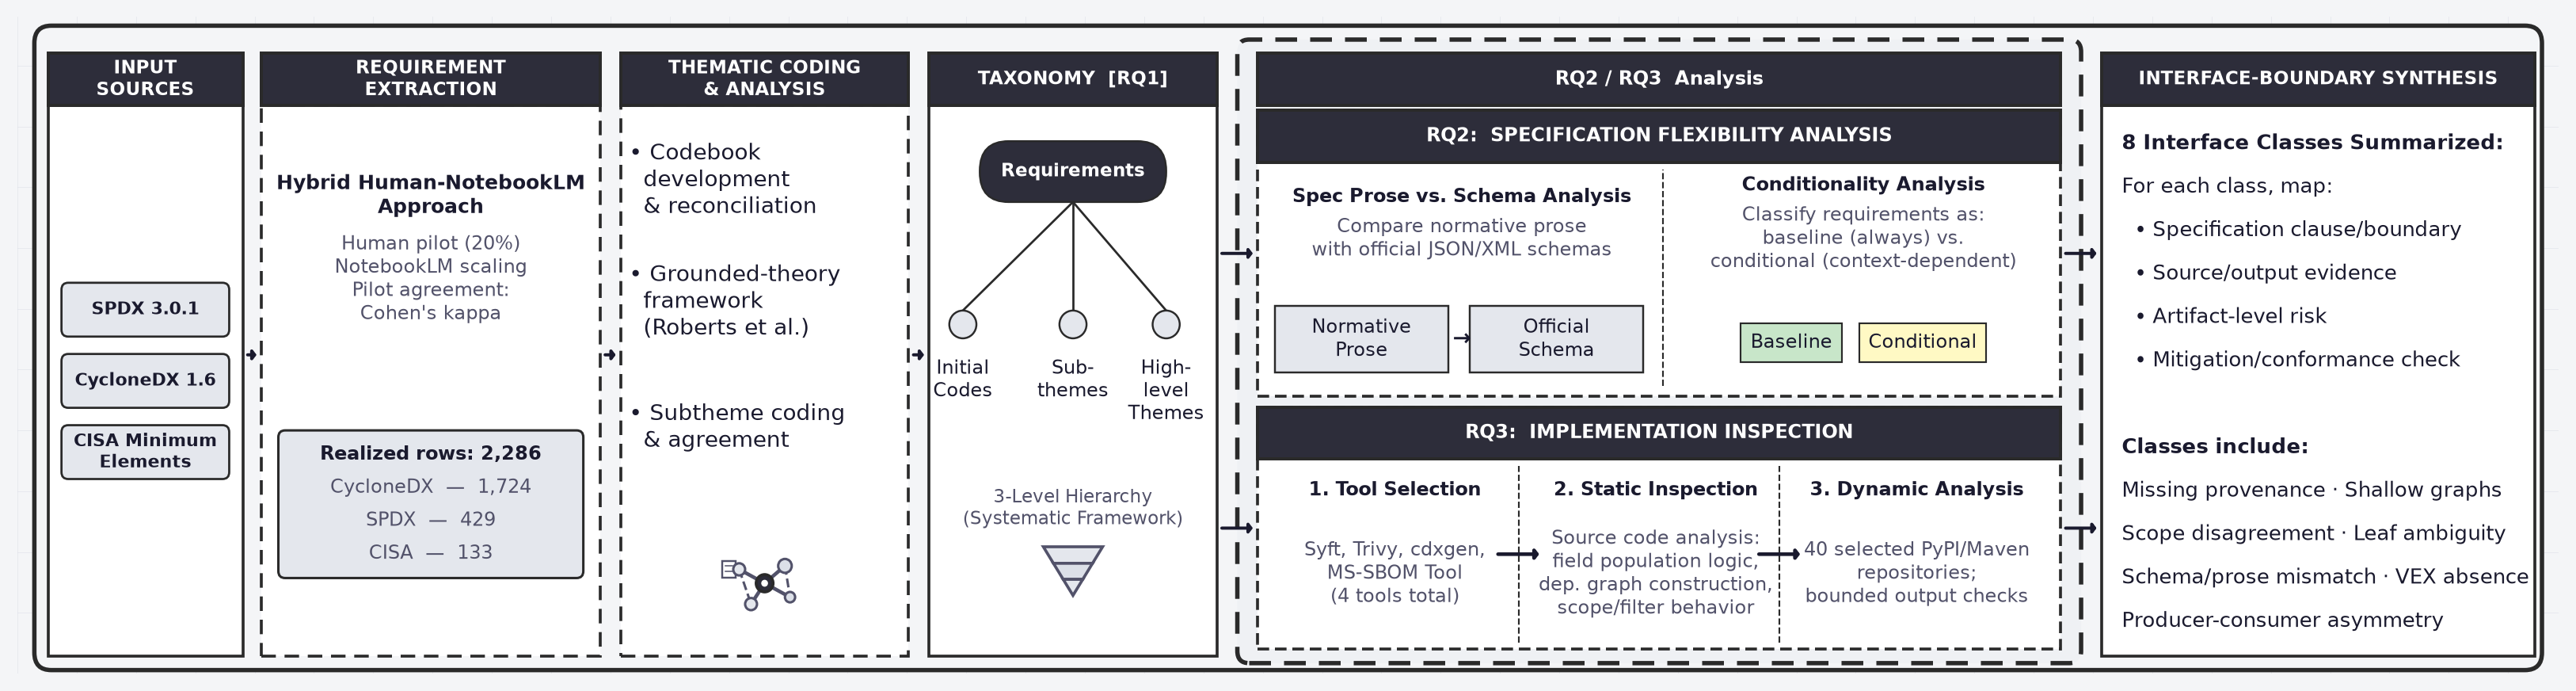
\includegraphics[width=\textwidth]{figures/methodology_pipeline.png}
\caption{Methodology pipeline; totals denote rows extracted under the stated protocol.}
\Description{Flowchart from three SBOM specification sources through requirement extraction, thematic coding, taxonomy construction, schema and conditionality analysis, four-tool implementation inspection, and synthesis into eight interface classes.}
\label{fig:req_analysis_pipeline}
\end{figure*}

Figure~\ref{fig:req_analysis_pipeline} connects specification text, generator implementations, and validation artifacts. RQ1 and RQ2 identify normative and structural boundaries; RQ3 traces selected boundaries through source and outputs.

\textbf{RQ1: What structural and semantic constraints do SBOM specifications impose on producers and consumers?}
We extract requirements from CycloneDX 1.6, SPDX 3.0.1, and CISA ME-SBOM. A requirement is a source statement or table unit constraining what a producer, consumer, document, or tool must, should, or may contain or do. Normative force follows RFC~2119-style \textit{MUST/REQUIRED}, \textit{SHOULD/RECOMMENDED}, and \textit{MAY/OPTIONAL} categories~\cite{rfc2119}.

\textbf{RQ2: To what extent do official schemas enforce the normative constraints defined in the specification prose, and where do they permit structural variation?}
We group requirements by purpose, compare normative prose with official schemas, and classify requirements activated only by optional classes, profiles, properties, or root objects.

\textbf{RQ3: How do generator tools implement the choices left open by specifications?}
We purposively inspect Syft and Trivy (both formats), cdxgen (CycloneDX), and Microsoft SBOM Tool (SPDX)~\cite{trivygithub,syftgithub,cdxgengithub,microsoftsbomtoolgithub}. All appear in prior empirical studies~\cite{reichmann2026poking,wangadherencegap2026}; the selection supports source-path comparison, not statistical sampling.

\subsection{Requirement Extraction}
We use a staged extraction process based on the grounded theory approach for analyzing technical guidelines \cite{chen2024}. A \emph{primary unit} is the smallest objective source segment evaluated for extraction: a complete sentence, list item, table row or cell, figure caption, or linked class/property definition. Annotators assign a binary decision to each unit, with 1 indicating that it contains at least one normative requirement and 0 indicating that it does not; a positive unit can yield multiple rows when it contains separable directives.

Two human annotators first applied this procedure independently to pilot samples covering 20\% of each specification, then reconciled disagreements. Cohen's Kappa in Table~\ref{tab:iar_kappa_scores} measures agreement on this binary extraction decision. We use $\kappa$ for the pilot because correctly agreeing to include requirement-bearing units and exclude non-normative units is part of establishing protocol reliability. Stage~1 agreement was lower for SPDX ($\kappa=0.458$) because its table-driven organization created boundary disagreements over whether a row, cell, or linked class definition constituted one primary unit. Because these disagreements included unitization, the Stage~1 score is a conservative consistency indicator rather than a strict chance-corrected estimate over a fixed unit set. After refining the unit-of-analysis and table-boundary rules, Stage~2 human agreement increased to $\kappa=0.820$ for SPDX, $0.827$ for CycloneDX, and $0.854$ for the CISA Minimum Elements for a Software Bill of Materials~\cite{cisaframing2024} (henceforth \textit{CISA ME-SBOM}).

The refined protocol was then scaled with Google's NotebookLM (accessed during July 2025). Human-to-NotebookLM agreement in Table~\ref{tab:iar_kappa_scores} uses the reconciled pilot material and measures the same binary primary-unit decision under the refined protocol.

After scaling, we conducted a held-out audit outside the 20\% pilot. For each specification, we randomly sampled 10\% of its pages from outside the pilot and divided them into the primary units defined above. Without viewing NotebookLM's output, the primary analyst independently applied the same binary extraction decision used in the pilot. Unlike the pilot's focus on protocol validation, this audit directly evaluates machine-extraction agreement on unseen source material using Cohen's Kappa. The resulting held-out agreement was $\kappa=0.922$ across 615 CycloneDX units and $\kappa=0.867$ across 52 CISA ME-SBOM units; the SPDX held-out score will be inserted after final verification. After scoring, a second analyst reviewed every disagreement with the primary analyst. This qualitative review found no major systematic omissions in the machine-extraction process and therefore did not alter the pre-reconciliation score.

The dataset contains 2,286 extracted rows: 1,724 from CycloneDX, 429 from SPDX, and 133 from CISA ME-SBOM. These totals describe the rows produced by the protocol, not a guaranteed exhaustive inventory. The CISA rows include directives about creation, exchange, lifecycle, framing, and data-field guidance, not 133 distinct minimum data fields.

Raw row counts are not directly comparable across specifications because specification structure affects the extraction unit. For example, CISA ME-SBOM expresses that a conformant tool needs to possess the mandatory data field ("Dependency Relationship"). The corresponding obligation is expressed in CycloneDX prose by the statement that a tool "should" populate the \texttt{dependencies} graph for every component, which we extract as one \texttt{SHOULD}-level row, and in SPDX as table rows describing the \texttt{Relationship} element and its permitted types. We use counts and percentages only for within-corpus description and audit navigation. Our clause-level conditionality, schema/prose, and implementation-trace arguments do not depend on the magnitude of the row totals.

Appendix~\ref{app:prompts} records the LLM extraction methodology and prompts used to scale the corpus. We retain the extraction files unchanged and treat them and the generated tables as auditable intermediate artifacts rather than reproducible ground truth. Exact regeneration is not guaranteed because NotebookLM is a closed, nondeterministic system. The final inventory and anonymous location of the supplementary archive remain marked in the artifact-availability statement.

\begin{table}[t]
\caption{Cohen's Kappa ($\kappa$) for Pilot Requirement-Extraction Agreement.}
\label{tab:iar_kappa_scores}
\centering
\resizebox{\columnwidth}{!}{%
\begin{tabular}{@{}llccc@{}}
\toprule
\textbf{Stage} & \textbf{Comparison} & \textbf{CycloneDX} & \textbf{CISA ME-SBOM} & \textbf{SPDX} \\
\midrule
Stage 1 & Human vs.\ Human & 0.732 & 0.779 & 0.458 \\
\midrule
\multirow{2}{*}{Stage 2}
    & Human vs.\ Human      & 0.827 & 0.854 & 0.82 \\
    & Human vs.\ NotebookLM & 0.782 & 0.815 & 0.75 \\
\bottomrule
\end{tabular}%
}
\par\smallskip
{\scriptsize\emph{Note:} The table reports pilot agreement; the post-scaling audit reports held-out kappa separately.}
\end{table}

\subsection{Thematic Coding}
\label{subsec:thematiccoding}

We interpreted the extracted requirements using a codebook-based thematic analysis following Roberts et al.~\cite{roberts2019attempting}:

\begin{enumerate}
\item \textbf{Codebook Development:} A primary analyst first coded a 20\% sample. During a sanity check, the analysts discussed ambiguous codes and category placement and agreed on consistent decision rules. The primary analyst then completed the full corpus, assigning each requirement to one subtheme, and formalized the resulting codebook with each subtheme's label and definition, inclusion/exclusion criteria, decision rules, and boundary examples. For example, \textit{Dependency Representation} includes requirements to record upstream/downstream component relationships and excludes component-identity requirements that name no relationship.
\item \textbf{Inter-Coder Agreement:} Using the finalized codebook, a secondary human annotator independently assigned one subtheme to each normative-requirement row in a stratified random sample targeting 25\% of each specification and spanning its sections. Agreement required an exact subtheme match with the primary analyst. Because each specification has a different subtheme codebook, we report within-specification exact percentage agreement rather than a pooled kappa. Pre-reconciliation agreement, calculated as $100\times A/(A+D)$~\cite{milesandhuberman1994,roberts2019attempting}, was 392/431 (91.0\%) for CycloneDX, 91/107 (85.0\%) for SPDX, and 28/34 (82.4\%) for CISA ME-SBOM. After recording these values, the annotators discussed every disagreement and assigned the final subtheme by consensus; reconciliation was not counted as initial agreement. This human-to-human thematic check is distinct from the requirement-extraction agreement in Table~\ref{tab:iar_kappa_scores}.

\end{enumerate}

After subtheme coding and reconciliation, semantically related subthemes were grouped into mutually exclusive high-level themes while retaining the underlying initial codes and subthemes; no subtheme was assigned to more than one high-level theme. For example, \texttt{dep\_graph\_population}, transitive-resolution, and dependency-scope codes form \textit{Dependency Representation} under \textit{Structural Completeness}. This labels structural-coverage requirements; it does not claim dependency ground truth.

For CycloneDX, the refined coding yields 13 merged subthemes and 7 final themes; for SPDX, 15 merged subthemes and 6 final themes; and for CISA ME-SBOM, 16 merged subthemes and 6 final themes. 

\subsection{Schema and Conditionality Analysis}
\label{subsec:schemaandconditionalityanalysis}
For schema analysis, we manually construct an expected schema based on the extracted normative requirements and compare it against the official machine-readable schemas. We classify mismatches into definition presence, property presence, property type, and requiredness/constraint differences. This comparison concerns machine-checkable structure; external dependency discovery, producer evidence coverage, and defensive-task sufficiency are evaluated through prose, profile, source, and output evidence rather than treated as JSON Schema obligations.

For conditionality, we construct a minimum template SBOM for each specification and map which requirements apply to that baseline. We then classify prerequisites for the remaining requirements, such as profile conformance, class instantiation, property presence, data type presence, serialization choice, or optional root-object inclusion. This measures the practical baseline enforced by the standard rather than the total size of the specification.

\subsection{Implementation Inspection}
\label{subsec:implementationinspection}
We combine manual source inspection with focused output validation. 

\textbf{Manual inspection.}
Fixed snapshots are Trivy v0.72.0, cdxgen v12.7.1, Syft v1.48.0, and Microsoft SBOM Tool v4.1.11; Table~\ref{tab:tool-evidence} records their exact commits, inspected formats, and source anchors. These snapshots define the evidence boundary and were re-verified in July 2026. They are not latest-release claims, and later versions would require reinspection. Following Chen et al.~\cite{chen2024}, we trace serialization entry points across provenance, component identity, dependency relationships, scope/filtering, and coverage/analysis signals. We record conditionality and surfaced omissions, requiring a repository-relative path for every source observation.

\textbf{Dynamic Generation.} To complement the static inspection, we conduct focused output validation across two package ecosystems: PyPI and Maven. For PyPI, we selected the top 20 packages by monthly download count, and for Maven, we selected the top 20 artifacts by reported usage rank, giving 40 selected packages in total \cite{pypistats, mvnrepository}. For each package we generated CycloneDX outputs with Syft, Trivy, and cdxgen, and SPDX outputs with Syft, Trivy, and the Microsoft SBOM Tool, aggregating one output per package per tool. This popularity-based set spans two ecosystems but is not statistically representative of
PyPI, Maven, or other ecosystems. We do not quantify inventory overlap, graph depth, reproducibility, or vulnerability-result variation; the artifacts provide bounded observations rather than frequency estimates or a comprehensive tool benchmark.

For the SPDX CISA-derived presence analysis, we operationalized ten valid checks: SBOM author, software producer, component name, software identifier, component hash, license, dependency relationship, tool name, timestamp, and generation context. We excluded a separate automated check labeled ``component version'' because it reads \field{CreationInfo.specVersion}, which records the document format version rather than a package's version. It is therefore a non-CISA document-format control and appears in neither the numerator nor denominator reported in Section~\ref{subsec:cisa-compliance}.

Our specification analysis (Section~\ref{sec:spec-analysis}) targets SPDX 3.0.1, but Trivy and Syft produce SPDX 2.3 natively. Their generation behavior therefore originates under SPDX 2.3, not under SPDX 3.0.1. We converted their native artifacts to SPDX 3.0.1 using the official SPDX Online Tools converter \cite{spdxonlinetools}, which wraps the SPDX Workgroup's reference Spdx2to3Converter, solely to obtain a common representation baseline. Conversion between major versions is a defined field-and-type mapping rather than a lossless transform, and prior work reports that conversion can reinterpret or drop fields \cite{sbomlandscape}; we do not infer that these tools' historical implementation choices were caused by SPDX 3.0.1.

\textbf{Conversion Fidelity Check}. For reported cross-version field-presence comparisons, we locate the corresponding field in the native 2.3 artifact and confirm whether its presence or absence remains visible after conversion. Any native/converted discrepancy is attributed to conversion and excluded from generator-level findings. This check supports representational comparability; it does not establish causal traceability from a 3.0.1 clause to a tool implemented for 2.3.

\subsection{Synthesis Output}
The evidence-chain synthesis links each boundary to its specification source, implementation/output observation, artifact-level risk, and mitigation without assigning a single cause.
 % - [merging 7/2]
\section{Specification Analysis}
\label{sec:spec-analysis}

\subsection{Thematic Structure}
The distributions show which obligation types dominate each extracted corpus, while clause mappings establish their normative force and schema enforcement. SPDX is profile-driven and graph-oriented: 57\% of its extracted rows are class-specific, mostly constraining structure rather than content. In CycloneDX (Table~\ref{tab:cdx_theme_distribution}), provenance, identity, and trust leads with 585 rows (33.9\%), followed by specialized security models with 397 (23.0\%); dependency and downstream-use semantics account for 32 (1.9\%). The mapped clauses show where a valid artifact may leave provenance, filtered dependencies, or empty graph entries unexplained.

\begin{tcolorbox}[colback=gray!4!white, colframe=black!80, boxrule=0.5pt, arc=5pt, left=2pt, right=2pt, top=1pt, bottom=1pt]
\textbf{Key Takeaway:} The extracted corpora emphasize structural and class-specific rules. Dependency coverage and explicit meanings for missing data receive less baseline guidance, creating the interface boundaries analyzed below.
\end{tcolorbox}

\subsection{CISA: Mandatory Process, Softer Data Quality}
\begin{figure}[t]
    \centering
    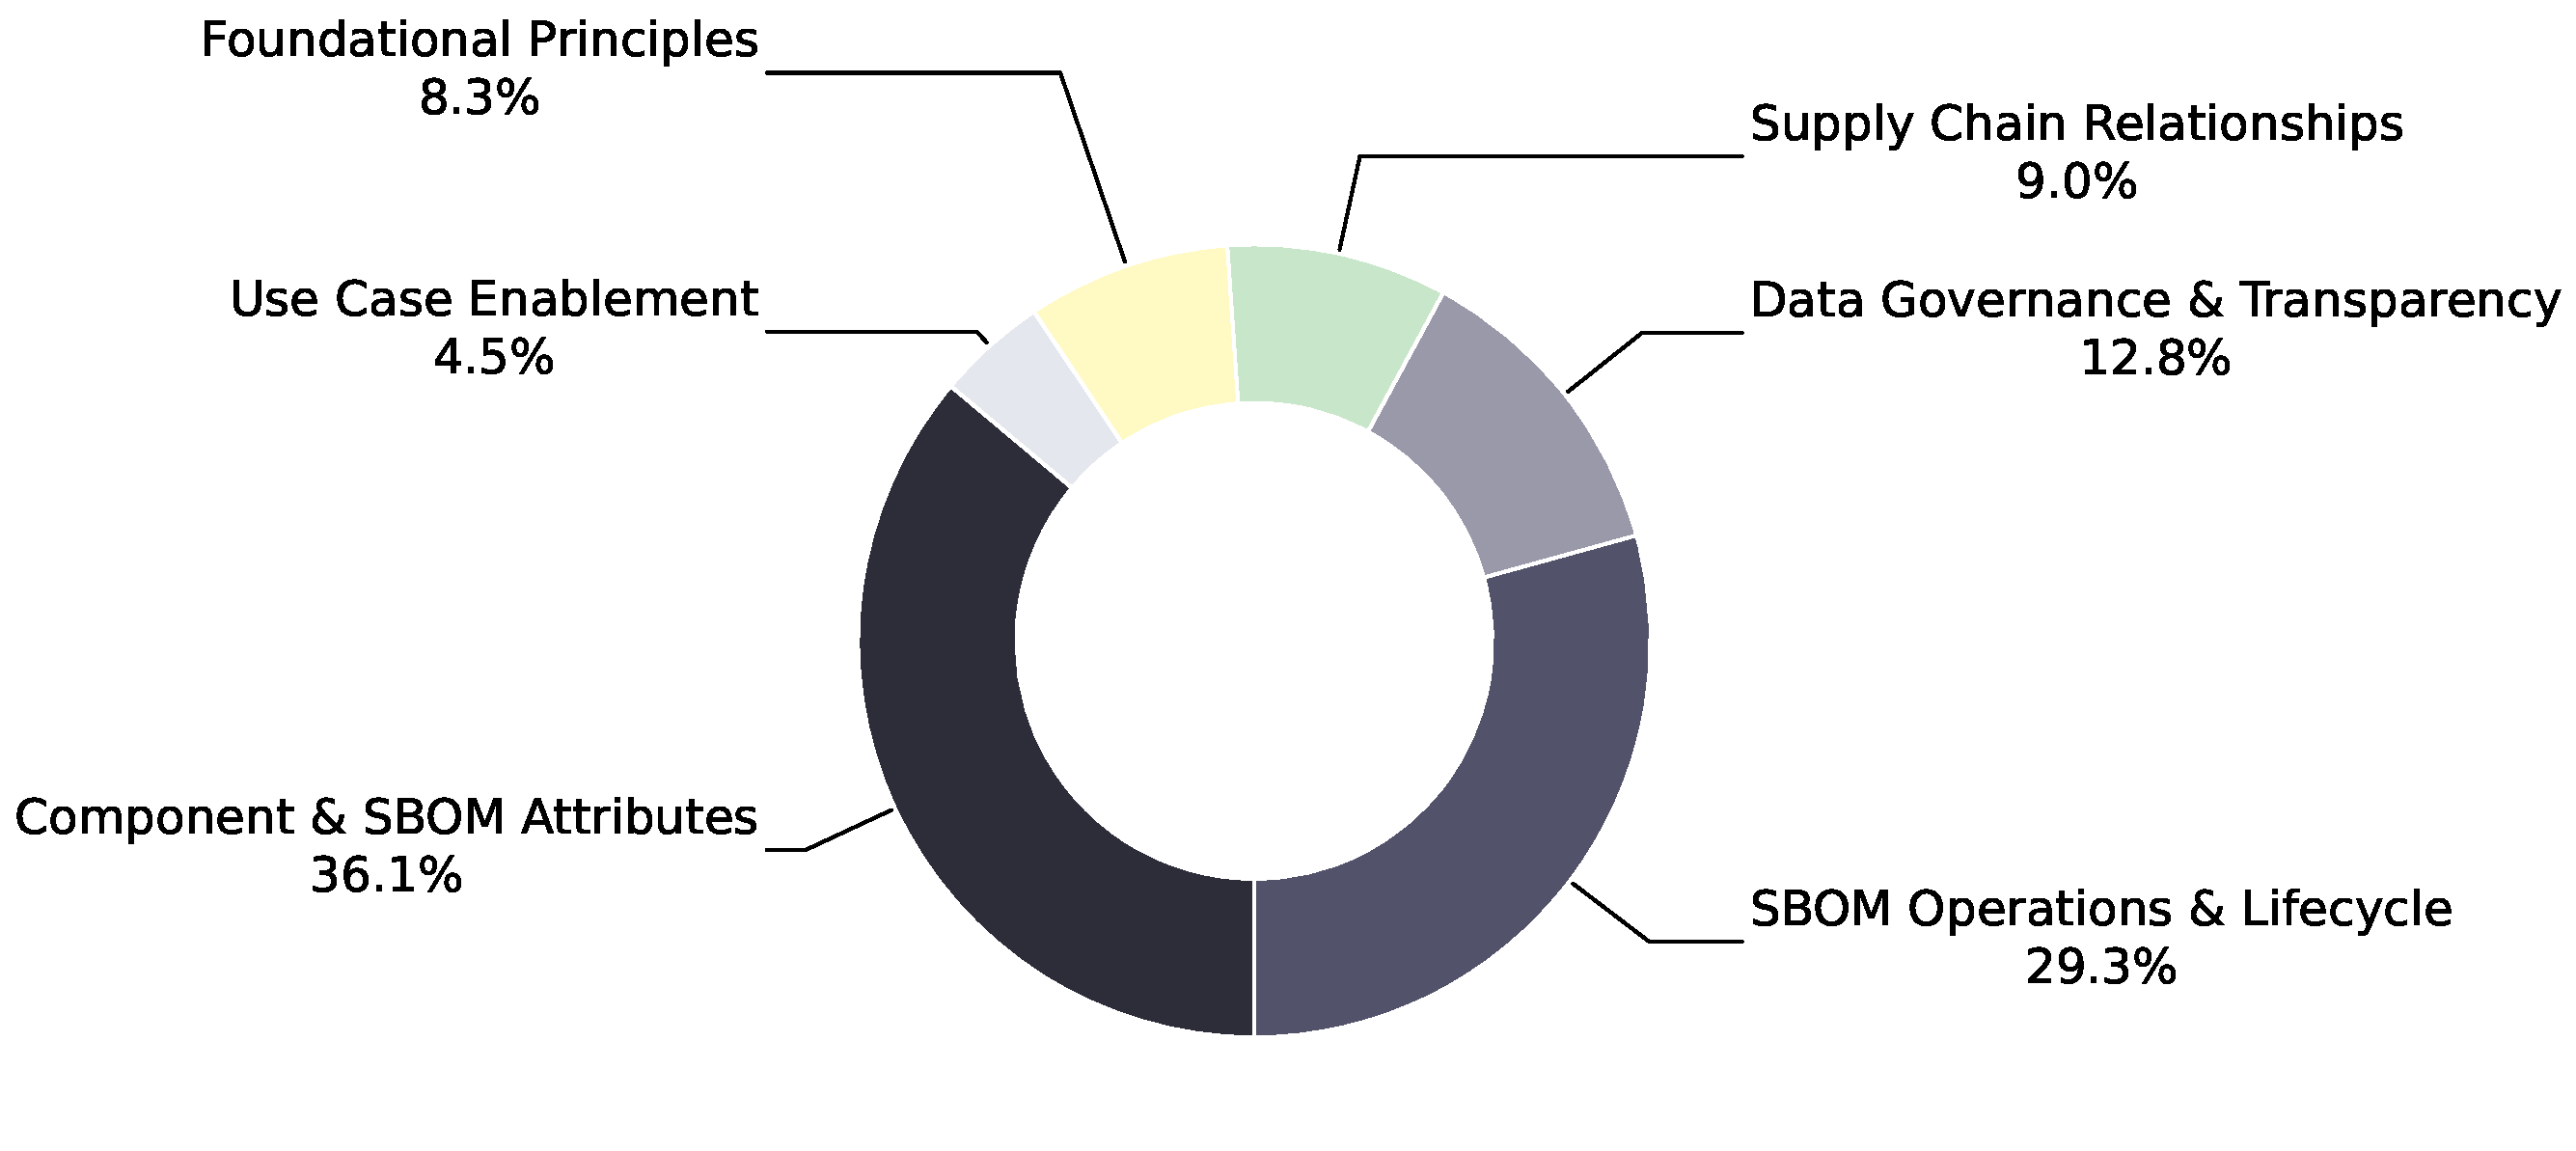
\includegraphics[width=\columnwidth]{figures/cisa_theme_pie.pdf}
    \vspace{-2.5em}
    \caption{CISA themes within the 133-row extracted corpus.}
    \Description{Pie chart of the 133 extracted CISA rows. Component and SBOM Attributes is the largest theme at 36.1 percent, followed by SBOM Operations and Lifecycle at 29.3 percent; the remaining rows are distributed among the other themes.}
    \label{fig:cisa_theme_distribution}
\end{figure}

CISA's operational minimum elements include supplier, author, component identity/version, dependency relationships, and timestamp. Its 133 extracted rows also cover creation, exchange, lifecycle, and framing; they are not 133 distinct fields. Component \& SBOM Attributes (36.1\%) and SBOM Operations \& Lifecycle (29.3\%) lead the distribution in Figure~\ref{fig:cisa_theme_distribution}. Clause-level coding shows stronger creation directives than some content-validation guidance, so process compliance can coexist with weak provenance or undeclared coverage. CycloneDX and SPDX represent CISA's fields, but baseline schema validity need not require them. SPDX 3.0.1's Lite Profile makes package \texttt{suppliedBy} and \texttt{packageVersion} mandatory, for example, only when producers declare and implement that profile.

\begin{tcolorbox}[colback=gray!4!white, colframe=black!80, boxrule=0.5pt, arc=5pt, left=2pt, right=2pt, top=1pt, bottom=1pt]
\textbf{Key Takeaway:} CISA-aligned profiles can require baseline supplier and version fields, but producers must declare and implement them. Schema validity without such a profile does not guarantee those fields or explain their absence.
\end{tcolorbox}

\subsection{SPDX: Strong Graph Structure, Limited Population Guidance}
SPDX 3.0.1 models dependencies as explicit \field{Relationship} edges such as \field{dependsOn}, but gives limited guidance on discovering and populating the graph.

\begin{table}[htbp]
\caption{SPDX theme distribution within the 429-row extracted corpus}
\label{tab:spdx_theme_distribution}
\centering
\footnotesize
\begin{tabular}{@{}ll@{}}
\toprule
\textbf{Theme} & \textbf{Percentage} \\
\midrule

\textbf{Legal Compliance and Licensing Governance} & \textbf{14}\% \\
\hspace{1.5em}Normative reference versioning & 1\% \\
\hspace{1.5em}License expression syntax & 3\% \\
\hspace{1.5em}Custom license text & 9\% \\

\textbf{Profile modularity and tool interoperability} & \textbf{25}\% \\
\hspace{1.5em}Mandatory profile isolation rules & 9\% \\
\hspace{1.5em}Minimal SBOM profile compliance & 16\% \\

\textbf{Data serialisation and document integrity} & \textbf{8}\% \\
\hspace{1.5em}Deterministic JSON serialisation & 5\% \\
\hspace{1.5em}Dual layer structural and semantic validation & 1\% \\
\hspace{1.5em}Cryptographic hash and content identifier enforcement & 2\% \\

\textbf{Provenance, identity, and dependency graphing} & \textbf{15}\% \\
\hspace{1.5em}Element identity and provenance tracking & 10\% \\
\hspace{1.5em}Explicit relationship cardinality and directionality rules & 4\% \\
\hspace{1.5em}Lifecycle scope parameterisation & 1\% \\

\textbf{Security, vulnerability, and vex response} & \textbf{25}\% \\
\hspace{1.5em}Vulnerability scoring and exploit probability standardisation & 13\% \\
\hspace{1.5em}Vex status relationship constraints & 12\% \\

\textbf{Universal identification and distributed resolution} & \textbf{13}\% \\
\hspace{1.5em}External identifier and cross-document mapping standards & 1\% \\
\hspace{1.5em}Package URL encoding standards & 11\% \\

\bottomrule
\end{tabular}
\par
{\scriptsize\emph{Note:} Within-corpus percentages; subtheme totals may differ due to rounding.}
\end{table}


\textbf{Qualitative results.} Only Core is mandatory among nine profiles; 69 of 429 extracted rows apply universally, while the rest depend on class instantiation or profile conformance (Table~\ref{tab:spdx_theme_distribution}). Modularity tailors artifacts but limits what baseline conformance guarantees. \textbf{Schema results.} Of 30 property-type differences, the schema was more lax in 14 cases (e.g., \texttt{oneOf} alternatives) and more restrictive in 16 (e.g., \texttt{allOf} regexes), creating implementation-relevant prose/schema boundaries.

\begin{tcolorbox}[colback=gray!4!white, colframe=black!80, boxrule=0.5pt, arc=5pt, left=2pt, right=2pt, top=1pt, bottom=1pt]
\textbf{Key Takeaway:} SPDX profiles tailor artifacts to specific use cases, while baseline conformance guarantees only Core. Declared use-case profiles and explicit absence reasons are needed to interpret unpopulated concepts.
\end{tcolorbox}

\subsection{CycloneDX: Expressive Security Model, Limited Baseline Requirements}
CycloneDX represents provenance, dependency coverage, VEX, and build evidence through \field{metadata}, \field{dependencies}, \field{compositions}, \field{vulnerabilities}, and \field{formulation}. Their optionality supports multiple BOM purposes, but absence may mean inapplicable, unknown, unsupported, filtered, intentionally omitted, or outside the profile. The root graph is optional, and direct/transitive coverage is recommended rather than baseline-required.

\begin{table}[t]
\caption{CycloneDX theme distribution within the 1,724-row extracted corpus}
\label{tab:cdx_theme_distribution}
\centering
\footnotesize
\begin{tabular}{@{}ll@{}}
\toprule
\textbf{Theme} & \textbf{Percentage} \\
\midrule

\textbf{Provenance, identity, and trust} & \textbf{33.9}\% \\
\hspace{1.5em}BOM identity and references & 16.2\% \\
\hspace{1.5em}Producer and document metadata & 12.2\% \\
\hspace{1.5em}Integrity metadata & 5.5\% \\

\textbf{Specialized security data models} & \textbf{23.0}\% \\
\hspace{1.5em}Specialized BOM extensions & 23.0\% \\

\textbf{Completeness and evidence} & \textbf{12.9}\% \\
\hspace{1.5em}Build provenance and evidence & 12.0\% \\
\hspace{1.5em}Completeness and evidence claims & 0.9\% \\

\textbf{Component inventory and identity} & \textbf{10.9}\% \\
\hspace{1.5em}External identifiers and references & 4.8\% \\
\hspace{1.5em}Component identity and metadata & 4.1\% \\
\hspace{1.5em}Legal and licensing metadata & 2.1\% \\

\textbf{Structural conformance and validation} & \textbf{10.1}\% \\
\hspace{1.5em}Extension and annotation mechanisms & 7.9\% \\
\hspace{1.5em}Document structure and conformance & 2.1\% \\

\textbf{Vulnerability and VEX semantics} & \textbf{7.3}\% \\
\hspace{1.5em}Vulnerability and VEX records & 7.3\% \\

\textbf{Dependency and downstream-use semantics} & \textbf{1.9}\% \\
\hspace{1.5em}Dependency and assembly semantics & 1.9\% \\

\bottomrule
\end{tabular}
\par
{\scriptsize\emph{Note:} Within-corpus percentages; subtheme totals may differ due to rounding.}
\end{table}


\textbf{Qualitative results.} Optional or permissive rows form 54.9\% of the 1,724-row corpus, a within-corpus statistic. \field{compositions} can declare coverage and \field{scope} distinguish required dependencies, but producers compute them from heterogeneous evidence. \textbf{Schema results.} The 38 granular mismatches include prose presence constraints absent from schema and undocumented strictness such as \field{additionalProperties = false}. Neither layer verifies external discovery or runtime truth.

For traceability, CycloneDX recommends direct/transitive coverage (\texttt{CDX-0008} and \texttt{CDX-0009}), makes root \field{dependencies} optional (\texttt{CDX-0029}), and requires empty entries once a graph is emitted (\texttt{CDX-0925}). Optional decision points include document-level \field{metadata.supplier} (\texttt{CDX-0052}), component scope (\texttt{CDX-0276}), compositions (\texttt{CDX-0938}), and formulation (\texttt{CDX-1256}). Section~\ref{sec:tool-analysis} traces these identifiers into source and output evidence.

\begin{tcolorbox}[colback=gray!4!white, colframe=black!80, boxrule=0.5pt, arc=5pt, left=2pt, right=2pt, top=1pt, bottom=1pt]
\textbf{Key Takeaway:} CycloneDX can represent provenance, dependency coverage, VEX, and build evidence. Declared use cases and absence reasons help consumers interpret which evidence an artifact includes.
\end{tcolorbox}

\subsection{Common Structural Ambiguities Across Specifications}
Across CISA, SPDX, and CycloneDX, optional constructs and external evidence leave three producer decisions open:

\textbf{Dependencies.} SPDX uses typed relationships; CycloneDX uses a reference-keyed root graph. Neither resolves discovery: producers choose whether to include development, optional, transitive, manual, or runtime packages.

\textbf{Vulnerabilities.} Both formats represent security exposure, but representation is not availability: an inventory-only SBOM can acquire vulnerability data later, so schema validity does not establish vulnerability context.

\textbf{Absence semantics.} Both formats provide scoped signals: SPDX's \texttt{NoAssertionElement} can record a non-assertion for particular relationships, while CycloneDX compositions can mark declared coverage incomplete or unknown~\cite{spdx301,ecma424}. Neither mechanism supplies a uniform vocabulary across provenance, filtering, vulnerability, and coverage fields, so an omitted optional field can still be ambiguous.

A schema-valid SBOM can answer ``is this shaped correctly?'' but not which evidence was covered, whether dependencies were filtered, or what absence means. Those questions require profiles, producer declarations, or external evidence.

\textbf{RQ1 and RQ2 synthesis.} For RQ1, the specifications precisely constrain the structure and relationships of instantiated elements, but leave many evidence-discovery, population, and absence-semantics decisions to producers and profiles. For RQ2, official schemas enforce many structural and type constraints on emitted elements; optional profiles, conditional prose, and external evidence boundaries require separate specification-conformance and use-case-sufficiency checks.

\begin{tcolorbox}[colback=gray!4!white, colframe=black!80, boxrule=0.5pt, arc=5pt, left=2pt, right=2pt, top=1pt, bottom=1pt]
\textbf{Key Takeaway:} SPDX and CycloneDX can express some known-unknown or incomplete states, but optional fields may still disappear without a reason. Schema validation alone cannot distinguish missing evidence from an intentional omission.
\end{tcolorbox}

\begin{table}[t]
\caption{Auditable source and output anchors for representative implementation claims.}
\vspace{-1em}
\label{tab:tool-evidence}
\centering
\scriptsize
\begin{tabularx}{\columnwidth}{@{}p{1.6cm}p{3.1cm}X@{}}
\toprule
\textbf{Snapshot / inspected format} & \textbf{Repository-relative source anchor} & \textbf{Inspected decision / output observation} \\
\midrule
Trivy v0.72.0\newline\emph{CycloneDX 1.6; SPDX 2.3}\newline\texttt{0c40a8d4b9b9} & \path{pkg/flag/package_flags.go} (\field{--include-dev-deps}); \path{pkg/scan/local/service.go} (\texttt{excludeDevDeps}); \path{pkg/sbom/io/encode.go} (\texttt{Encoder.Encode}) & Default development-dependency filtering precedes emission; 18/18 outputs met the empty-entry rule, and 0/18 declared \field{compositions}. \\
cdxgen v12.7.1\newline\emph{CycloneDX 1.6}\newline\texttt{70e7a729b10d} & \path{lib/cli/index.js} (\texttt{buildBomNSData}); \path{lib/stages/postgen/postgen.js} (\texttt{filterBom}) & Dependency-entry construction/optional filtering; 13 applicable outputs lacked empty entries, and 0/18 declared \field{compositions}. \\
Syft v1.48.0\newline\emph{CycloneDX 1.6; SPDX 2.3}\newline\texttt{e9e34948534a} & \path{syft/format/common/cyclonedxhelpers/to_format_model.go} (\texttt{isExpressiblePackageRelationship}; \texttt{toDependencies}) & Maps expressible package dependencies; 3 applicable outputs lacked empty entries (15 N/A). \\
Microsoft SBOM Tool v4.1.11\newline\emph{SPDX 3.0.1}\newline\texttt{e47d1d4b1f37} & \path{src/Microsoft.Sbom.Parsers.Spdx30SbomParser/Generator.cs} (\texttt{GenerateJsonDocument}); \path{src/Microsoft.Sbom.Api/Workflows/Helpers/RelationshipsArrayGenerator.cs} (\texttt{GenerateAsync}) & Constructs creation metadata, \field{suppliedBy}, and typed relationships; output did not declare Lite. \\
\bottomrule
\end{tabularx}
\end{table}
 % 3 [inter spec b/w c and s - 7/1]
\section{Tool Implementation Analysis}
\label{sec:tool-analysis}

\begin{table*}[t]
\caption{Representative interface boundaries and mitigation checks.}
\label{tab:root-causes}
\centering
\footnotesize
\begin{tabularx}{\textwidth}{@{}p{2.2cm}p{3.1cm}p{3.6cm}p{3.4cm}X@{}}
\toprule
\textbf{Inconsistency} & \textbf{Specification source} & \textbf{Inspected source/output evidence} & \textbf{Downstream risk} & \textbf{Mitigation/check} \\
\midrule
Missing provenance & Metadata fields exist but are not always baseline-required & Trivy and cdxgen differ on document-level author/metadata-supplier population; Microsoft SBOM Tool constructs creation metadata and package \field{suppliedBy}, using \field{NOASSERTION} when supplier input is unavailable & The artifact may not reliably identify the SBOM author, document-level metadata supplier, or component/package supplier & Require level-specific supplier, author, timestamp, and tool identity in task-specific defensive profiles \\
\addlinespace
Shallow dependency graph & Direct/transitive coverage is recommended or conditional, not always mandatory & Inspected snapshots expose different graph-construction and filtering paths & An artifact-only inventory check cannot assess an omitted dependency & Compare declared evidence sources with component-to-graph coverage; use depth only as a diagnostic; require coverage status \\
\addlinespace
Ambiguous leaf nodes & Empty dependency entries do not distinguish a true leaf from unsupported graph recovery & Trivy emits empty entries for no dependencies, with implementation ambiguity acknowledged & The artifact does not distinguish unknown coverage from producer-asserted complete coverage & Add a graph-confidence or coverage-status assertion for empty dependency entries \\
\addlinespace
Scope disagreement & Scope/runtime relevance is representable but computation is not specified & cdxgen infers scope; Trivy filters development dependencies before output & The same project can yield different required/optional dependency sets & Require generators to declare evidence source and filtering policy \\
\addlinespace
Relationship model loss & Internal tool relationships may not map cleanly to an output format & Syft maps only expressible package dependency relationships into CycloneDX dependencies & The artifact may omit evidence or containment relationships used during generation & Report relationship classes that were dropped, converted, or represented outside the dependency graph \\
\addlinespace
Producer-consumer asymmetry & Many requirements describe producer-populated fields; fewer define absence meaning & Inspected paths omit or infer fields based on local evidence and options & The artifact does not distinguish inapplicable, unknown, unsupported, filtered, intentionally omitted, or profile-excluded data & Standardize machine-readable absence states for provenance, dependency, vulnerability, and coverage fields \\
\addlinespace
Undeclared optional features & Formulation, VEX analysis, and compositions are optional root objects & No evaluated CycloneDX output declared \field{compositions}; cdxgen formulation is opt-in & The artifact may not state whether a feature is irrelevant, unavailable, or outside its intended use & Define use-case profiles plus explicit absence states for provenance, dependency, VEX, and coverage claims \\
\addlinespace
Schema/prose mismatch & Schemas may be stricter, looser, or structurally different from prose & Schemas provide machine-executable structural constraints & A schema-valid artifact may still violate an applicable prose obligation & Add versioned schema/prose structural-diff tests; assign evidence checks to profiles or external validation \\
\bottomrule
\end{tabularx}
\end{table*}

Specification flexibility becomes consequential when generators translate project evidence into concrete SBOM fields. Using the dual methodology described in Section~\ref{sec:methodology}, we inspected frozen snapshots of Microsoft SBOM Tool, cdxgen, Trivy, and Syft. Static claims are limited to those snapshots; CycloneDX and SPDX output counts are limited to 40 selected PyPI and Maven package repositories per tool, and SPDX presence/gap results to the evaluated artifacts. Our objective is not to benchmark or rank tools, but to document where selected implementation choices and output patterns align with the specification boundaries identified in Section~\ref{sec:spec-analysis}. The results cover CISA-derived field presence (\S\ref{subsec:cisa-compliance}), selected schema-gap criteria (\S\ref{subsec:security-gaps}), and static design choices (\S\ref{subsec:static-inspection}).

\subsection{CISA Compliance: Dynamic Validation}
\label{subsec:cisa-compliance}
This analysis evaluates whether the selected SPDX and CycloneDX artifacts populate the CISA-derived fields defined in Section~\ref{subsec:implementationinspection}. Both formats provide vocabulary for these fields, but the evaluated artifacts do not populate every criterion consistently.

\subsubsection{SPDX Generators}
Within the evaluated SPDX artifacts from the three generators, 4 of the 10 valid CISA-derived checks were populated in every output: software identifier, dependency relationship, tool name, and timestamp. The ten-field operationalization is defined in Section~\ref{subsec:implementationinspection}. We exclude the former ``component version'' result because its automated check read \field{CreationInfo.specVersion}, a document-format property, rather than a package-version field.

For the Trivy and Syft artifacts, we compared the ten CISA-derived fields used in Section 5.1.1 between the native SPDX 2.3 output and its converted SPDX 3.0.1 representation. We observed no presence/absence discrepancies for those fields. This scoped check was not a full-document conversion audit and does not establish lossless conversion for unexamined fields, types, or relationships.

SPDX 3.0.1's Lite Profile provides a mechanism for reducing minimum-element ambiguity, but its benefits depend on adoption. The evaluated Microsoft 3.0.1 output did not declare Lite Profile conformance, while Trivy and Syft emitted 2.3 natively, so these outputs do not test the effect of implementing the Lite Profile.

Even among these consistently present fields, the evaluated artifacts used different representations. For instance, the CISA-defined ``Tool Name'' field maps to SPDX's \texttt{createdUsing}, which mandates only an identifier, not a human-readable string. We observed both explicit URIs (e.g., \texttt{http://trivy.dev/}) and opaque hashes, so resolving basic tool identity from the artifact can require graph dereferencing. Tool identity is a core element of SBOM provenance, but the identifier alone does not directly communicate whether a generator is trusted or audited. We did not test whether or how downstream consumers perform this resolution.

\subsubsection{CycloneDX Generators}
Table~\ref{tab:cdx-schema-gap} (Appendix~\ref{app:prompts}) aggregates outputs from the 40 selected PyPI and Maven package repositories per tool. A tool-level criterion is \emph{Met} only when every applicable study output meets it, \emph{Unmet} when at least one applicable output does not, and \emph{N/A} only when no output exercises the construct. For all-component rules, one component lacking the field makes that output Unmet.

The four tool-level Unmet patterns have different force. First, cdxgen omitted required empty graph entries in 13 outputs with a dependency graph (five had no graph and were N/A); Syft did so in 3 applicable outputs (15 N/A), while all 18 Trivy outputs met this prose rule. Second, the CISA-derived document-level \field{metadata.supplier} criterion was Unmet for every output from all three tools; this says nothing about component-level supplier population. A source repository may also lack authoritative product-supplier evidence, so the result establishes field absence in the artifacts, not a generator defect. Third, the all-component version criterion was Unmet in 2 of 18 cdxgen outputs, all 18 Syft outputs, and 5 of the 6 Trivy outputs containing components (12 Trivy outputs had no components and were N/A). This means at least one component lacked a version, not that every component did. Fourth, no output used the optional \field{compositions} element to declare coverage status. The supplier and version rows are CISA-derived checks and compositions is advisory; their Unmet status is not a schema-validity judgment. Only the empty-entry result tests an applicable mandatory CycloneDX prose rule omitted from schema enforcement.

\begin{tcolorbox}[colback=gray!4!white, colframe=black!80, boxrule=0.5pt, arc=5pt, left=2pt, right=2pt, top=1pt, bottom=1pt]
\textbf{Key Takeaway:} In the selected CycloneDX outputs, no tool populated document-level supplier or declared compositions, and every tool had outputs with at least one missing component version. Representing a field does not ensure that generators populate it.
\end{tcolorbox}

\subsection{Security-Relevant Schema Gaps: Prose Beyond Validation}
\label{subsec:security-gaps}
We test whether executable schemas enforce selected prose obligations whose data supports provenance and dependency-aware security analysis. These are structural checks, not vulnerability tests: a schema can validate shape while leaving graph coverage or field population unenforced.

\subsubsection{SPDX 3.0.1}
All selected rules exercised by the three SPDX outputs passed, as detailed in Table~\ref{tab:spdx-schema-gap} (Appendix~\ref{app:prompts}). N/A rows mark constructs that were not emitted; they are not failures or evidence about how those constructs would behave. This control result supports only the checked emitted constructs, not broader SPDX conformance.


\subsubsection{CycloneDX 1.6}
CycloneDX shows the consequential gap. Once a dependency graph is emitted, \texttt{CDX-0925} requires an entry for every component, including an empty \field{dependsOn} list for leaves; the schema does not enforce that coverage. Thirteen applicable cdxgen outputs and three Syft outputs omitted at least one required empty entry. These artifacts can remain schema-valid, yet schema validation alone cannot tell a dependency-aware consumer whether a component is an asserted leaf or its graph status was not reported. We did not test downstream vulnerability decisions.

\begin{tcolorbox}[colback=gray!4!white, colframe=black!80, boxrule=0.5pt, arc=5pt, left=2pt, right=2pt, top=1pt, bottom=1pt]
\textbf{Key Takeaway:} The selected checks passed for every exercised SPDX construct. In CycloneDX, 13 cdxgen and 3 Syft outputs omitted required empty dependency entries that the schema does not enforce, leaving graph-coverage status ambiguous for dependency-aware security analysis.
\end{tcolorbox}

\subsection{Static Inspection: Generator Design Choices}
\label{subsec:static-inspection}
Static inspection traces how the frozen generator snapshots implement filtering, provenance, graph construction, and relationship translation within the boundaries identified by the specification analysis.

\textbf{Evidence chain 1: filtered dependency coverage.} CycloneDX \texttt{CDX-0008} and \texttt{CDX-0009} recommend rather than require direct and transitive coverage, while \texttt{CDX-0927} recommends a composition assertion when graph coverage is unknown. Trivy makes \field{--include-dev-deps} opt-in and filters development packages and edges before graph encoding (Table~\ref{tab:tool-evidence}). All 18 evaluated outputs satisfied the applicable empty-entry rule, but none declared \field{compositions}. An artifact-only check can therefore observe the emitted graph but cannot determine whether omitted development dependencies were filtered, undiscovered, or absent. This bounded ambiguity does not establish inventory inaccuracy, consumer effects, or a sole cause; product priorities, package metadata, configuration, and defects remain possible explanations.

Trivy also records tool identity and timestamps and can populate component-level \field{components[].supplier} from package metadata, but the inspected path does not populate a document-level author or \field{metadata.supplier}. This distinction matters because CISA-style provenance separates the emitting tool, SBOM author, document-level metadata supplier, and component suppliers.

\textbf{Evidence chain 2: mandatory prose beyond schema enforcement.} Once a CycloneDX graph is emitted, \texttt{CDX-0925} requires an empty \field{dependsOn} entry for components with no known dependencies, but the JSON schema does not enforce component-to-entry coverage. cdxgen constructs dependency entries and can rebuild them under optional filtering (Table~\ref{tab:tool-evidence}); required-only filtering was not enabled in the study. Nevertheless, 13 applicable outputs lacked at least one required empty entry, while five outputs without a graph were N/A. These artifacts can remain schema-valid while violating the applicable prose rule. A missing entry does not prove that a dependency itself was omitted, and consumer interpretation was not tested.

cdxgen separately exposes specification-permitted policy controls: it can propagate required scope, retain required components, and add an incomplete \field{compositions} assertion when filtering occurs. Component scope is optional under \texttt{CDX-0276}, and the 18 default study outputs contained no composition assertions. Formulation data under \texttt{CDX-1256} is likewise opt-in. These observations show that cdxgen can represent filtering policy under particular options; they do not establish that the standard caused the default-output pattern.

\textbf{Syft} provides a shorter translation trace. Its CycloneDX conversion admits package dependency relationships but not other internal relationship classes into the dependency graph (Table~\ref{tab:tool-evidence}), so the output can be narrower than the internal evidence model. Three applicable outputs lacked required empty entries, while 15 were N/A; this does not establish that relationship translation caused those failures. Component-supplier population is conditional on source metadata and does not populate the document-level \field{metadata.supplier} evaluated above.

\textbf{Microsoft SBOM Tool} is a scoped contrast, not a generally stronger tool. Its inspected path constructs \field{CreationInfo.createdBy}, \field{createdUsing}, package \field{suppliedBy}, and typed SPDX relationships (Table~\ref{tab:tool-evidence}). However, absent supplier input becomes \field{NOASSERTION}, not a verified identity, and the evaluated SPDX 3.0.1 document declared Core, Software, and Simple Licensing profiles but not Lite. The aggregate 4-of-10 result across three SPDX generators does not show that this Microsoft output populated every remaining field, so we make no overall conformance, evidence-coverage, or superiority claim.

\begin{tcolorbox}[colback=gray!4!white, colframe=black!80, boxrule=0.5pt, arc=5pt, left=2pt, right=2pt, top=1pt, bottom=1pt]
\textbf{Key Takeaway:} The inspected generators make different choices about dependency filtering, graph construction, provenance, and relationship translation. Their outputs do not consistently declare those policies, so consumers cannot reconstruct them from the artifact alone.
\end{tcolorbox}

\subsection{Synthesis: Valid Choices, Invisible Decisions}
Outputs reflect interacting specification latitude, ecosystem evidence, configuration, priorities, and defects. Our narrower finding is that some decisions are not declared: a missing supplier may be inapplicable, unknown, unsupported, filtered, intentionally omitted, unpopulated, or outside the declared profile. This is an artifact-information limit, not observed consumer behavior.

\textbf{RQ3 synthesis.} In the selected snapshots and artifacts, open boundaries appear as different provenance defaults, dependency filtering and graph construction, relationship translation, and coverage-status signaling. The source traces and focused output checks show choices the formats can represent or do not prevent; they neither apportion causality among standards, defects, priorities, evidence, and configuration nor estimate prevalence across the wider tool ecosystem.

\begin{tcolorbox}[colback=gray!4!white, colframe=black!80, boxrule=0.5pt, arc=5pt, left=2pt, right=2pt, top=1pt, bottom=1pt]
\textbf{Key Takeaway:} Schema validity confirms structure, not evidence coverage or fitness for a defensive task. Declared evidence sources, filters, coverage, and absence reasons let consumers assess those properties.
\end{tcolorbox}
 % 4 [merging results + analysis, 7/2]
\section{Interface Boundaries and Recommendations}
\label{sec:root-causes}

Table~\ref{tab:root-causes} presents representative, not exhaustive, evidence chains linking a corpus clause or requirement identifier to a source/output observation and artifact-level interface mismatch. It does not assign blame or map every behavior to one permissive clause; defects, priorities, package-manager evidence, and configuration remain competing or interacting explanations.

To make these recommendations implementable, we propose a cumulative three-level defensive conformance-check suite. This remains a design proposal derived from our findings; implementation and evaluation are future work.

\noindent\textbf{Level 1: Identity and provenance.} Profile-specific schema and field-presence rules can check machine-readable supplier/author, component name and version, identifier, timestamp, and tool identity. Anchors include CycloneDX \field{metadata.supplier}, \field{metadata.timestamp}, \field{metadata.tools}, and component identity fields, and SPDX \field{CreationInfo.createdBy}, \field{createdUsing}, \field{packageVersion}, and \field{suppliedBy}.

\noindent\textbf{Level 2: Evidence and coverage.} Profile rules can combine producer declarations with checks for evidence sources, filtering policy, dependency relationships, coverage status, and absence reasons. CycloneDX \field{dependencies}, \field{scope}, and \field{compositions}, together with SPDX relationships and declared profiles, provide machine-readable anchors; evidence-source, filtering, and absence declarations require profile rules or extensions where no standard field exists.

\noindent\textbf{Level 3: Defensive-task sufficiency.} Task-specific checks can evaluate vulnerability/VEX context and build/formulation evidence through CycloneDX \field{vulnerabilities[].analysis} and \field{formulation} or SPDX Security and Build profiles. They then compare the artifact's claims with external manifests, lockfiles, builds, containers, or runtime evidence for vulnerability response, compliance, or incident triage.

Schemas can check the machine-expressible structure at each level, but they cannot establish the truth of producer declarations. The levels therefore keep specification completeness, generator-evidence completeness, and security-use-case sufficiency separate. Passing a lower level does not establish a higher one, and graph depth remains a diagnostic rather than a stand-alone completeness measure.
 % 4, 5 [7/2]
\section{Discussion}
\label{sec:discussion}

\subsection{SBOM Inconsistency as an Interface Problem}
The main lesson from our analysis is that SBOM inconsistency is an interface problem. Optionality is not itself a defect: multi-use specifications legitimately support different disclosure constraints, ecosystems, and maturity levels. Consumer-facing ambiguity arises when the resulting artifact declares neither its use-case profile nor whether missing data is inapplicable, unknown, unsupported, filtered, intentionally omitted, or not required. A missing dependency graph or supplier field can reflect any of these states. Our study documents this ambiguity in specifications and generated artifacts; it does not observe how particular consumers interpret it.

Prior work establishes output inconsistency; our contribution maps selected differences that coexist with validation to open population rules and concrete generator decision points.

The SPDX schema-gap result also bounds this claim. The evaluated outputs passed every selected rule exercised by an emitted construct. N/A marks optional constructs that were not exercised and provides no evidence about their correctness. Thus our evidence distinguishes an observed applicable-rule violation from a feature that was simply not activated.

Because generators also depend on metadata conventions, package managers, build/runtime environments, and configuration, the result is an engineering interface assessment rather than sole-cause attribution. It identifies which evidence, filtering, and coverage claims require structural, profile-level, or external checks.

\subsection{Threats to Validity}
\textbf{Interpretation and coding.} Extraction and thematic coding require judgment. Pilot agreement, reconciliation, documented rules, and the independent check support reproducible subtheme assignment; the higher-level taxonomies remain auditable study artifacts, with community validation left to future work.

\textbf{Corpus coverage.} Pilot agreement established consistency under the refined extraction protocol. A random page-based audit outside the pilot measures human-to-NotebookLM agreement on unseen source material using the same binary primary-unit decision. The subsequent analyst review shows that disagreements can reflect either missed prescriptive directives or overly inclusive human labels; neither the kappa score nor the review establishes exhaustive extraction coverage. The central findings rest on mapped clauses, schemas, source paths, and outputs rather than row-count magnitude.

\textbf{Empirical scope.} Static findings concern the named frozen tool snapshots; dynamic checks use selected outputs generated from 40 repositories across PyPI and Maven for each supported tool and format. These popularity-based cases support mechanism-level traces, not tool rankings or population estimates; broader ecosystems and probabilistic sampling remain future validation.

\textbf{Consumer and evidence scope.} We analyze specifications, generators, and artifacts rather than downstream implementations or vulnerability outcomes. Accordingly, downstream statements identify bounded operational risks, while inventory completeness, build provenance, runtime loading, and defensive-task sufficiency require external evidence; graph depth alone is not a completeness measure.

\textbf{SPDX comparability.} Trivy and Syft generate SPDX 2.3 natively. Conversion provides a 3.0.1 representation baseline for selected fields, so cross-version claims are limited to field visibility under the mapping and do not attribute those tools' behavior to SPDX 3.0.1.
 % all [7/3]
\section{Conclusion}
\label{sec:conclusion}

SBOM specifications can accept structurally valid artifacts while leaving important generator choices unclear to consumers. In the evaluated CycloneDX outputs, the mandatory empty-dependency-entry rule was not schema-enforced and was violated by 13 applicable cdxgen outputs and 3 Syft outputs. No evaluated CycloneDX output populated document-level supplier metadata or declared composition-based coverage. The selected SPDX rules produced no Unmet result, providing a useful control: emitted constructs satisfied those checks, while N/A constructs were simply not exercised. Across both formats, profiles and rich data models represent provenance, relationships, vulnerabilities, build context, and coverage, but they do not provide a uniform cross-field vocabulary for explaining absent data.

The paper contributes a 2,286-row requirement corpus and clause-to-source-to-output evidence chains that support the cumulative suite in Section~\ref{sec:root-causes}. Level~1 checks identity and provenance, Level~2 checks evidence, filtering, coverage, and absence, and Level~3 evaluates vulnerability/VEX and build context against task needs. The four frozen snapshots and generated SBOMs trace these mechanisms rather than estimate ecosystem-wide prevalence. Implementing the suite and measuring consumer outcomes remain future work.
 % all [7/3]

%%
%% Acknowledgments (optional)
%%
\begin{acks}
The authors thank the anonymous reviewers for their constructive feedback.
\end{acks}

%%
%% Ethics and Privacy Statement
%%
\section*{Ethics and Privacy Statement}
This work does not involve human subjects or personal data. The analysis is based entirely on publicly available specifications (CycloneDX, SPDX, CISA guidance) and open‑source SBOM generation tools. We do not foresee any direct societal risks beyond those inherent in software supply chain security research.

%%
%% Bibliography – using ACM Reference Format
%%
\bibliographystyle{ACM-Reference-Format}
\bibliography{references}

%%
%% Appendices
%%
\appendix
\section{Supplementary Material}
\label{app:prompts}

This appendix provides supplementary materials that support the core analysis of the paper. First, it details the methodologies and prompts supplied to the NotebookLM assistant for the systematic extraction of normative requirements from the CISA, CycloneDX, and SPDX specifications. The main paper uses these prompts as provenance for the requirement corpus. Second, it presents the complete, tabulated results of our schema-gap tests, which compare generator outputs against the structural constraints defined by the specifications.
 
\subsection{Methodology for CISA Extraction}

The following text was provided to the LM as a source document named \texttt{SBOM\_Extraction\_Methodology.txt} to define the extraction rules.

\begin{tcolorbox}[breakable, colback=gray!4!white, colframe=black!80, fonttitle=\footnotesize, title=System Prompt: CISA Extraction Methodology, left=3pt, right=3pt, top=2pt, bottom=2pt, boxrule=0.5pt, arc=2pt]
\tiny
\vspace{-1em}
You are an expert assistant trained in the analysis of cybersecurity and software documentation, with a focus on Software Bills of Materials (SBOMs) and federal software supply chain policy.

You will be given sections of the CISA document titled \emph{“Framing Software Component Transparency: Establishing a Common Software Bill of Materials (Third Edition)”}. Your task is to analyze the content and extract \textbf{actionable directives} that relate to how SBOMs should be structured, formatted, or composed.

\textbf{Methodology:}
\begin{enumerate}
\item Read the document text carefully.
\item Extract statements that:
  \begin{itemize}
    \item Express explicit or strongly implied \textbf{requirements, recommendations, or aspirational goals}.
    \item Prescribe or suggest \textbf{what SBOMs should contain}, how they should be formatted, or how their elements should be related.
    \item Reflect \textbf{normative guidance}, even if phrased softly (e.g., “it is best to...”).
  \end{itemize}
\item Break compound statements into separate rows if each part contains a different actionable point.
\item Assign a Normative Keyword:
  \begin{itemize}
    \item Use the keyword verbatim if present.
    \item If not, infer:
      \begin{itemize}
        \item Minimum Expected → \texttt{MUST} or \texttt{REQUIRED}
        \item Recommended Practice → \texttt{SHOULD} or \texttt{RECOMMENDED}
        \item Aspirational Goal → \texttt{MAY} or \texttt{OPTIONAL}
      \end{itemize}
  \end{itemize}
\item Exclude purely descriptive statements, definitions, and examples.
\end{enumerate}

\textbf{Output Format:}  
A structured table with columns:
\begin{itemize}
  \item Section ID \& Heading
  \item Recommendation / Requirement
  \item Normative Keyword
\end{itemize}
Use exact text where possible.
\vspace{-1em}
\end{tcolorbox}

\noindent\textbf{Example CISA Prompt:}
\vspace{-0.4em}
\begin{tcolorbox}[colback=gray!4!white, colframe=black!80, boxrule=0.5pt, left=3pt, right=3pt, top=2pt, bottom=2pt, arc=2pt]
\tiny
\vspace{-0.8em}
\texttt{Using the system methodology in the source "SBOM\_Extraction\_Methodology", extract recommendations from the source "SBOM Framing... 2024" only from sections 'X' and 'Y'. Output a table: Section ID | Statement | Normative Keyword.}
\vspace{-0.8em}
\end{tcolorbox}

\subsection{Methodology for CycloneDX Extraction}

\begin{tcolorbox}[breakable, colback=gray!4!white, colframe=black!80, fonttitle=\footnotesize, title=System Prompt: CycloneDX Extraction Methodology, left=3pt, right=3pt, top=2pt, bottom=2pt, boxrule=0.5pt, arc=2pt]
\tiny
\vspace{-1em}
You are an expert research assistant specializing in the formal analysis of technical standards. Your task is to analyze the provided ECMA-424 source document and extract all \textbf{actionable directives} according to the following strict methodology.

\textbf{Core Methodology:}
\begin{enumerate}
\item Identify Actionable Directives: Any statement defining a rule (obligation, recommendation, or permission), including keywords like \texttt{MUST}, \texttt{SHOULD}, \texttt{MAY}, \texttt{Required}, or \texttt{Optional}. Treat \texttt{Optional} as actionable.
\item Synthesize Directives from Tables: For each table row, combine Property Name, Requirement Status, and Description to form a full directive.
\item Construct Requirement Text:
  \begin{itemize}
  \item GOOD: “The ‘metadata’ property is Optional.”
  \item BAD: “Property: metadata (Optional)”
  \end{itemize}
\item Extract Raw Keyword: Report the exact, verbatim keyword.
\item Exclude purely descriptive text, historical notes, or non-actionable examples.
\end{enumerate}

\textbf{Output Format (Mandatory):}  
A single Markdown table with columns:
\begin{itemize}
  \item Section ID \& Heading
  \item Recommendation / Requirement
  \item Normative Keyword
\end{itemize}
\vspace{-1em}
\end{tcolorbox}

\noindent\textbf{Example CycloneDX Prompt:}
\vspace{-0.4em}
\begin{tcolorbox}[colback=gray!4!white, colframe=black!80, boxrule=0.5pt, left=3pt, right=3pt, top=2pt, bottom=2pt, arc=2pt]
\tiny
\vspace{-0.8em}
\texttt{Using the methodology from the provided text, extract all actionable directives from ECMA-424.pdf. Analyze only content from Section X through Section Y. Provide the output as a Markdown table.}
\vspace{-0.8em}
\end{tcolorbox}

\subsection{Methodology for SPDX Extraction}

\begin{tcolorbox}[breakable, colback=gray!4!white, colframe=black!80, fonttitle=\footnotesize, title=System Prompt: SPDX Extraction Methodology, left=3pt, right=3pt, top=2pt, bottom=2pt, boxrule=0.5pt, arc=2pt]
\tiny
\vspace{-1em}
You are an expert research assistant specializing in the formal analysis of technical standards and software supply chain documentation.

You will be given sections of the SPDX 3.0.1 specification. Your task is to extract all actionable directives that constrain SPDX documents, classes, profiles, properties, relationships, or serialization behavior.

\textbf{Core Methodology:}
\begin{enumerate}
\item Extract statements containing explicit normative language such as \texttt{MUST}, \texttt{SHOULD}, \texttt{MAY}, \texttt{required}, \texttt{optional}, cardinality constraints, or profile conformance requirements.
\item Treat tables, class definitions, property cardinalities, and profile-specific constraints as normative when they define required or optional structure.
\item Break compound requirements into separate rows when they constrain different classes, profiles, relationships, or properties.
\item Preserve enough context to identify the relevant SPDX class, property, relationship type, profile, or serialization rule.
\item Exclude purely descriptive examples unless the example introduces a constraint not stated elsewhere.
\end{enumerate}

\textbf{Output Format (Mandatory):}
A table with columns:
\begin{itemize}
  \item Section ID \& Heading
  \item Recommendation / Requirement
  \item Normative Keyword
\end{itemize}
\vspace{-1em}
\end{tcolorbox}

\noindent\textbf{Example SPDX Prompt:}
\vspace{-0.4em}
\begin{tcolorbox}[colback=gray!4!white, colframe=black!80, boxrule=0.5pt, left=3pt, right=3pt, top=2pt, bottom=2pt, arc=2pt]
\tiny
\vspace{-0.8em}
\texttt{Using the extraction methodology, analyze only the SPDX 3.0.1 sections for the Software, Core, Security, and Lite profiles. Extract each actionable directive as a separate row with section context, requirement text, and normative keyword.}
\vspace{-0.8em}
\end{tcolorbox}

\subsection{Schema-Gap Test Results}

\vspace{-1.4em}
\begin{table}[ht]
\centering
\tiny
\caption{Selected Schema-Gap Criteria Across Three SPDX SBOMs}
\vspace{-1.4em}
\label{tab:spdx-schema-gap}
\begin{tabular}{llccc}
\toprule
Sec. & Rule & Microsoft & Syft & Trivy \\
\midrule
6.1.7  & DictionaryEntry keys unique          & N/A  & N/A  & N/A  \\
6.1.9  & Collection satisfies Core implicitly & Met & Met & Met \\
6.1.9  & element $\geq$1 implies rootElement  & Met & Met & Met \\
6.1.9  & element not of type SpdxDocument      & Met & Met & Met \\
6.1.9  & rootElement not of type SpdxDocument  & Met & Met & Met \\
6.1.21 & beginRange $\leq$ endRange            & N/A  & N/A  & N/A  \\
6.1.22 & NoneElement exclusive in ``to''       & N/A  & N/A  & N/A  \\
6.1.22 & NoAssertionElement usage in ``to''    & N/A  & N/A  & N/A  \\
6.4.1  & NoAssertionElement intent match       & N/A  & N/A  & N/A  \\
6.4.2  & NoneElement intent match              & N/A  & N/A  & N/A  \\
7.1.2  & File.name present                     & Met & Met & N/A  \\
7.1.3  & Package.name present                  & Met & Met & Met \\
\midrule
\multicolumn{2}{r}{Totals (Met/Unmet/N/A)} & 6/0/6 & 6/0/6 & 5/0/7 \\
\bottomrule
\end{tabular}
\par\smallskip
{\scriptsize Met/Unmet denotes whether the study rule held; N/A denotes an absent, unexercised construct.}
\end{table}

\FloatBarrier

\vspace{-1.4em}

\begin{table}[H]
\centering
\tiny
\caption{Selected Criteria Across CycloneDX Generator Outputs}
\vspace{-1.4em}
\label{tab:cdx-schema-gap}
\begin{tabular}{llccc}
\toprule
Sec. & Rule & cdxgen & Syft & Trivy \\
\midrule
Dependencies & Empty graph entries                 & Unmet & Unmet & Met \\
Identity     & PURLs structurally valid            & Met & Met & Met \\
Provenance   & Document metadata supplier (CISA)   & Unmet & Unmet & Unmet \\
Provenance   & Metadata timestamp (CISA)           & Met & Met & Met \\
Provenance   & Metadata tools (CISA)               & Met & Met & Met \\
Inventory    & Component names (CISA)              & Met & Met & Met \\
Inventory    & Component versions (CISA)           & Unmet & Unmet & Unmet \\
Inventory    & Component bom-refs                  & Met & Met & Met \\
Vulnerabilities & VEX analysis if vulns present  & N/A  & N/A  & N/A  \\
Completeness & Compositions assertion present      & Unmet & Unmet & Unmet \\
\midrule
\multicolumn{2}{r}{Totals (Met/Unmet/N/A)} & 5/4/1 & 5/4/1 & 6/3/1 \\
\bottomrule
\end{tabular}
\par\smallskip
{\scriptsize Cells aggregate 18 outputs/tool: Met requires every applicable output; one unmet applicable output yields Unmet; N/A requires no output to exercise the construct. These are study criteria, not schema-validity judgments.}
\end{table}


\end{document}
\endinput
